
\begin{figure}

    \centering
    \textbf{MATLAB}\hspace{8em}
    \textbf{Original}\hspace{8em}
    \textbf{Python}
    

    \begin{subfigure}{\textwidth}
        \centering
        
        \textbf{\rotatebox[origin=c]{90}{RMHL}}\begin{subfigure}{\textwidth}
        \centering
        
        \hspace{-3em}
        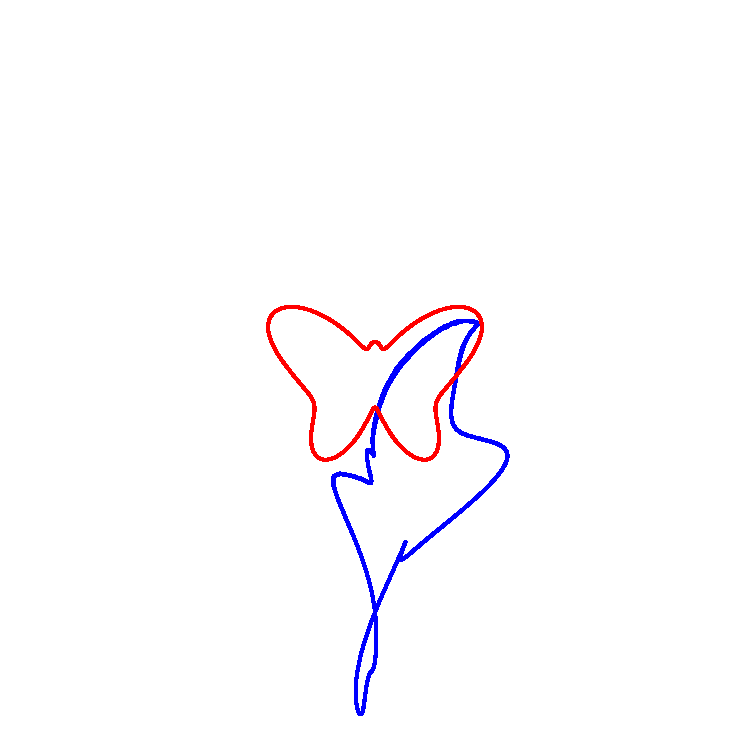
\includegraphics[trim=3cm 0cm 3cm 4cm, clip=true,height=.25\linewidth]{Figures/Fig_T3/MATLAB/RMHL_T2_Seg2_Trajectory.eps}
        \hspace{2em}
        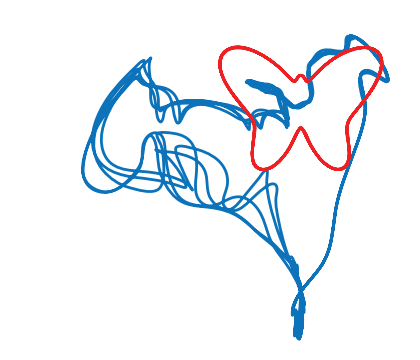
\includegraphics[trim=1cm 0cm 0cm 0cm, clip=true,height=.25\linewidth]{Figures/Fig_T3/Orig/RMHL_T2_Trajectory.png}
        \hspace{3em}
        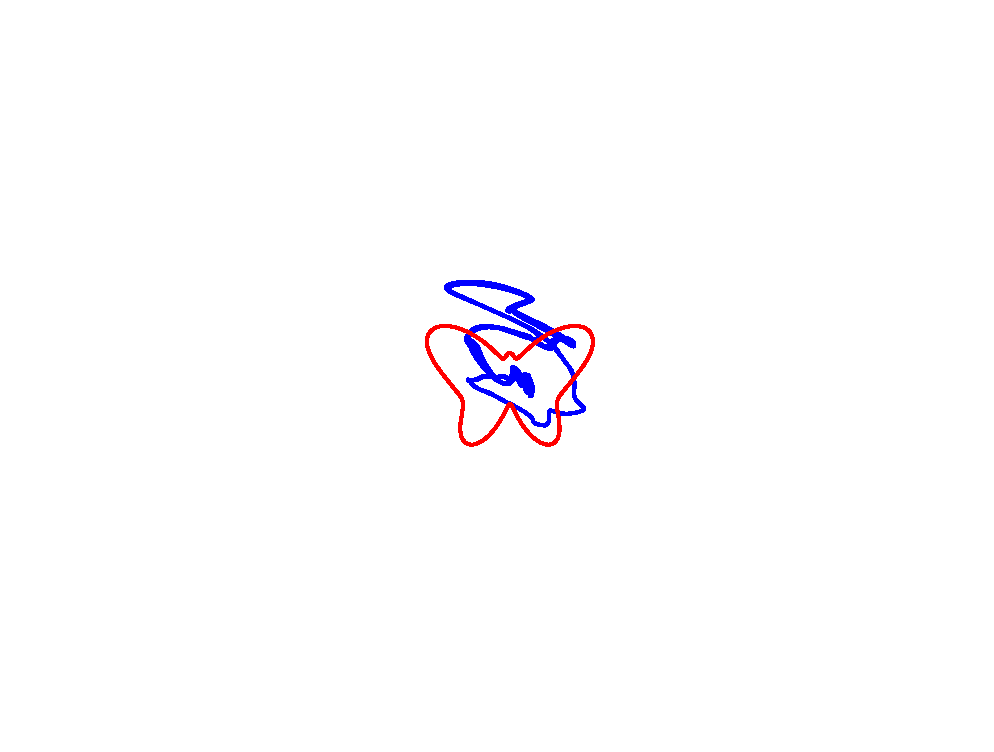
\includegraphics[trim=6cm 1.25cm 6cm 4.25cm, clip=true,height=.25\linewidth]{Figures/Fig_T3/Python/RMHL_T2_Seg2_Trajectory.eps}
        
        \end{subfigure}
         
        
        \textbf{\rotatebox[origin=c]{90}{$\theta_1$}}\begin{subfigure}{\textwidth}
        \centering
        
        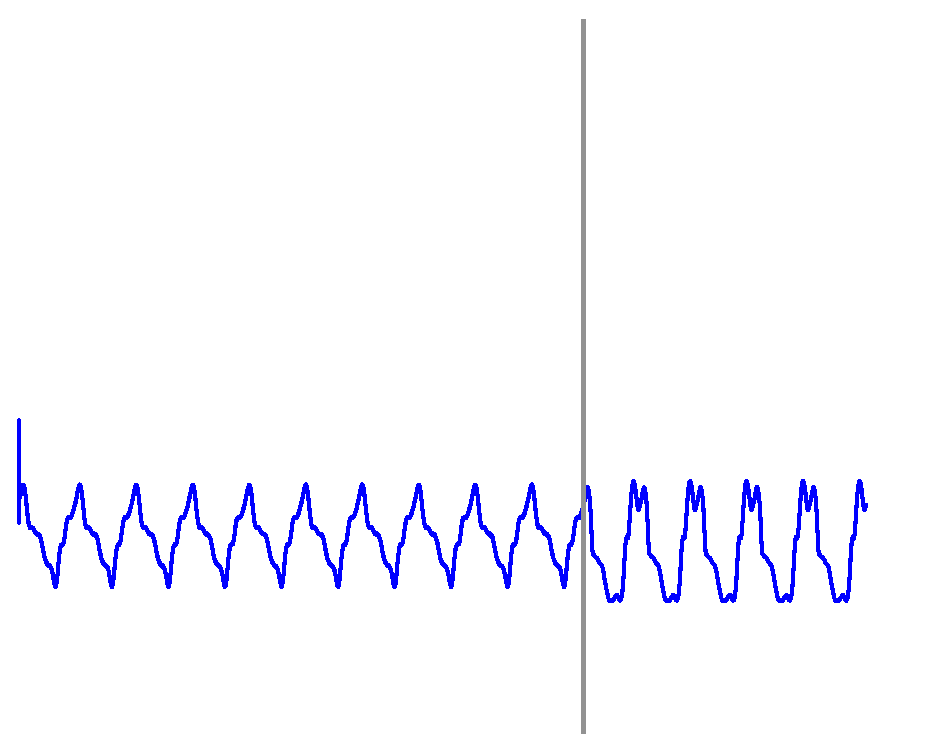
\includegraphics[height=0.1\linewidth,width=.45\linewidth]{Figures/Fig_T3/MATLAB/RMHL_T2_Seg2_Theta0.eps}
        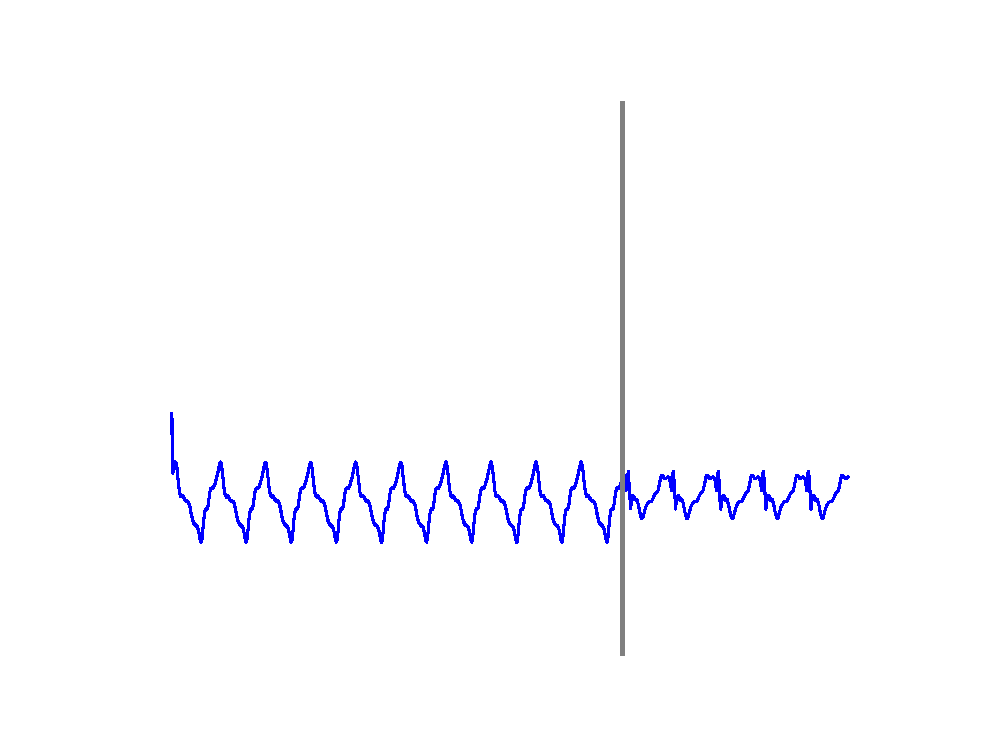
\includegraphics[trim=2cm 1cm 2cm 1cm, clip=true,height=0.1\linewidth,width=.45\linewidth]{Figures/Fig_T3/Python/RMHL_T2_Seg2_Theta0.eps}
        
        \end{subfigure}
         
        
        \textbf{\rotatebox[origin=c]{90}{$\theta_2$}}\begin{subfigure}{\textwidth}
        \centering
        
        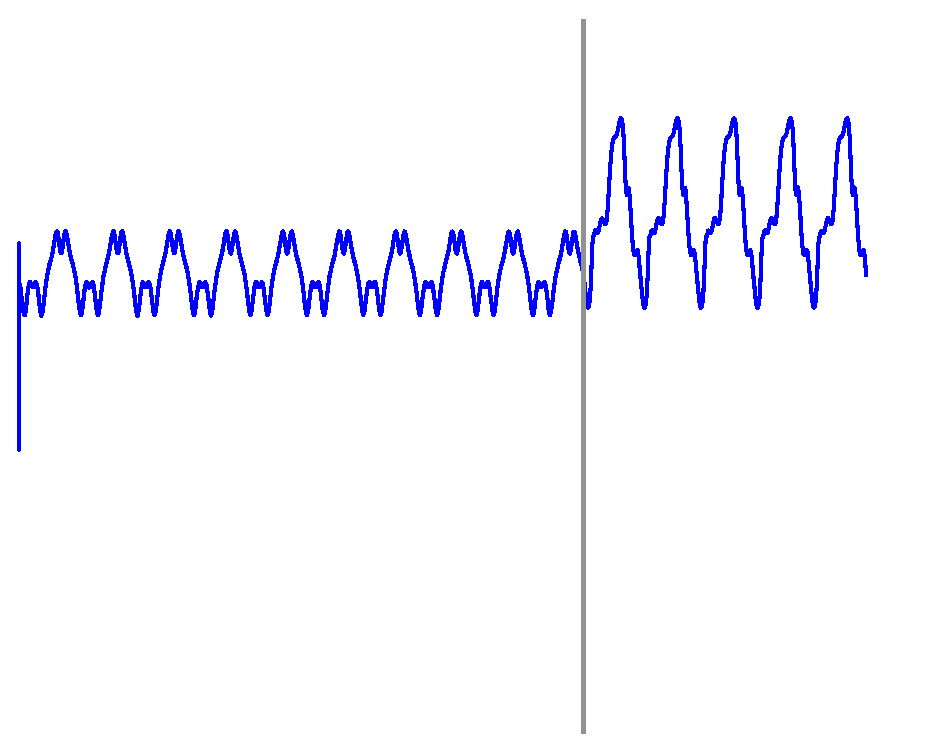
\includegraphics[height=0.1\linewidth,width=.45\linewidth]{Figures/Fig_T3/MATLAB/RMHL_T2_Seg2_Theta1.eps}
        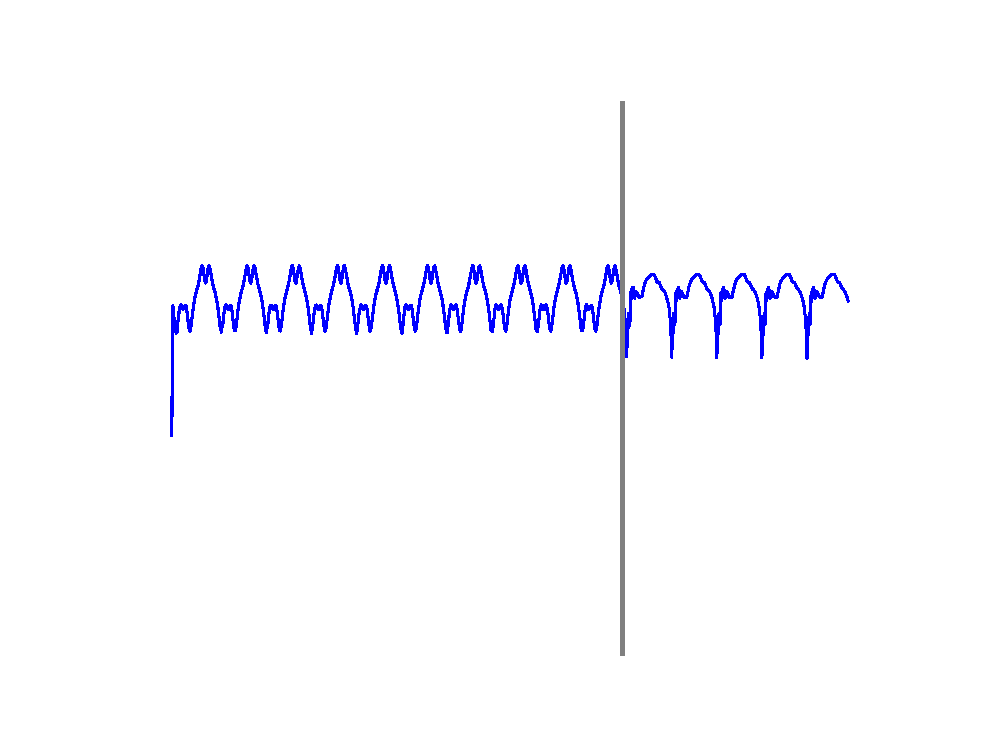
\includegraphics[trim=2cm 1cm 2cm 1cm, clip=true,height=0.1\linewidth,width=.45\linewidth]{Figures/Fig_T3/Python/RMHL_T2_Seg2_Theta1.eps}
        
        \end{subfigure}
         
        
        \textbf{\rotatebox[origin=c]{90}{MSE}}\begin{subfigure}{\textwidth}
        \centering
        
        \hspace{-2em}
        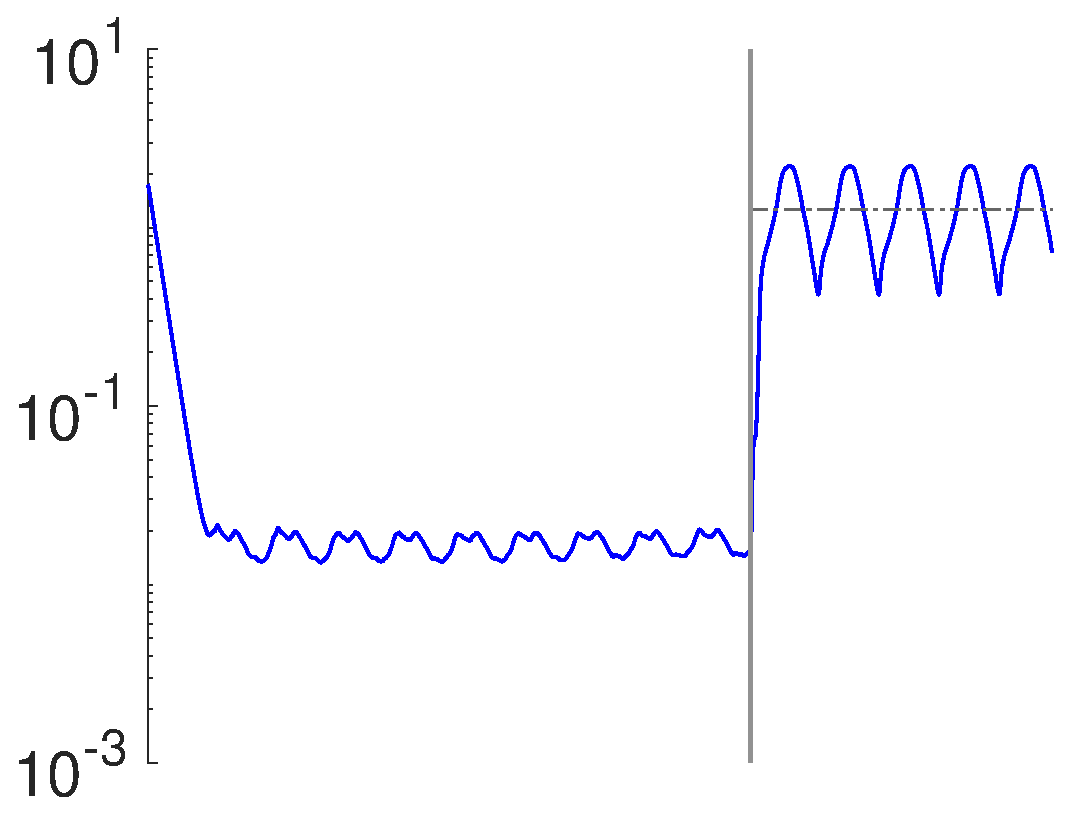
\includegraphics[height=0.15\linewidth,width=.45\linewidth]{Figures/Fig_T3/MATLAB/RMHL_T2_Seg2_MSE.eps}
        \hspace{.5em}
        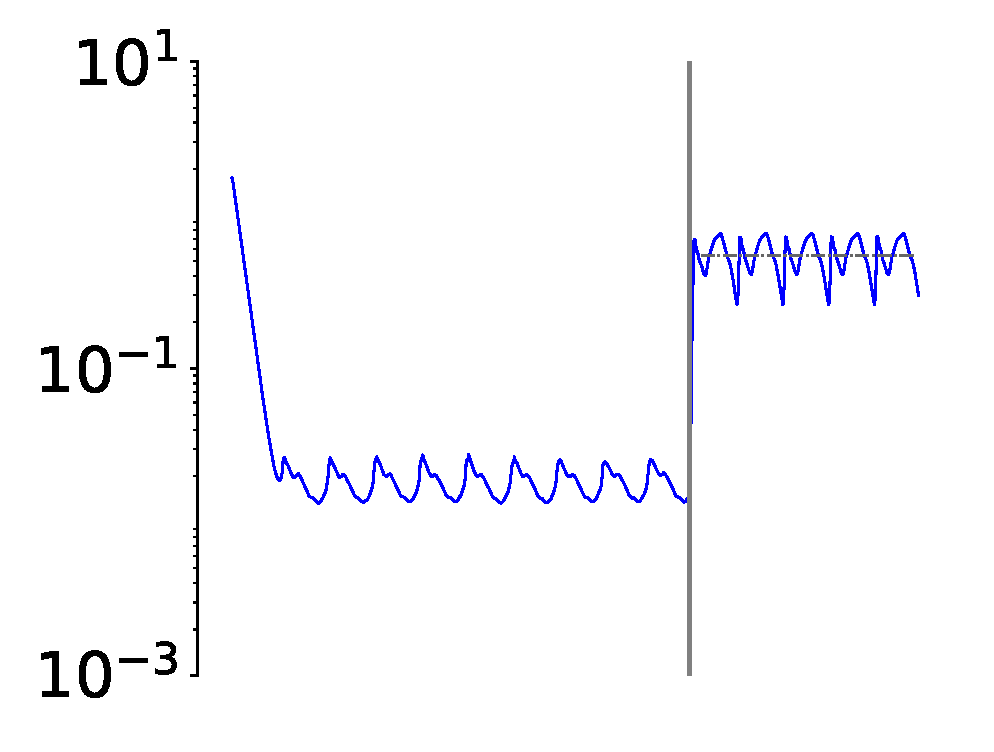
\includegraphics[height=0.15\linewidth,width=.45\linewidth]{Figures/Fig_T3/Python/RMHL_T2_Seg2_MSE.eps}
        
        \end{subfigure}
        
    \caption{Results for Task 2 with the RMHL algorithm. The target time‐series is imitated well by the model during the training phase (not shown), however, it is unable to maintain the time-series in a stable manner during the testing phase, in both implementations, as presented in \cite{pyle2019}.}
    \label{Fig:compTask2RMHL}
    \end{subfigure}
    
    \begin{subfigure}{\textwidth}
        \centering
        
        \textbf{\rotatebox[origin=c]{90}{SUPERTREX}}\begin{subfigure}{\textwidth}
        \centering
        
        
\includegraphics[trim=4cm 4cm 4cm 4.5cm, clip=true,height=.2\linewidth]{Figures/Fig_T3/MATLAB/ST_T2_Seg2_Trajectory.eps}
        \hspace{2em}
        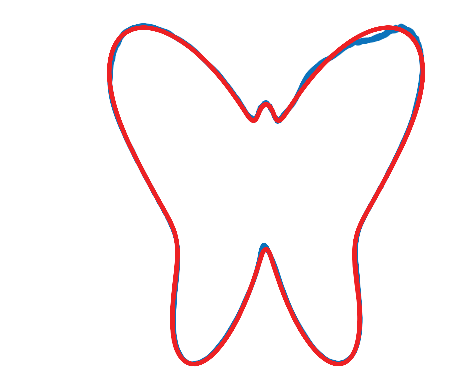
\includegraphics[trim=1cm 0cm 0cm 0cm, clip=true,height=.2\linewidth]{Figures/Fig_T3/Orig/ST_T2_Trajectory.png}
        \hspace{0em}
        
\includegraphics[trim=6cm 4.5cm 6cm 5cm, clip=true,height=.2\linewidth]{Figures/Fig_T3/Python/ST_T2_Seg2_Trajectory.eps}
        
        \end{subfigure}
        
        
        \textbf{\rotatebox[origin=c]{90}{$\theta_1$}}\begin{subfigure}{\textwidth}
        \centering
        
        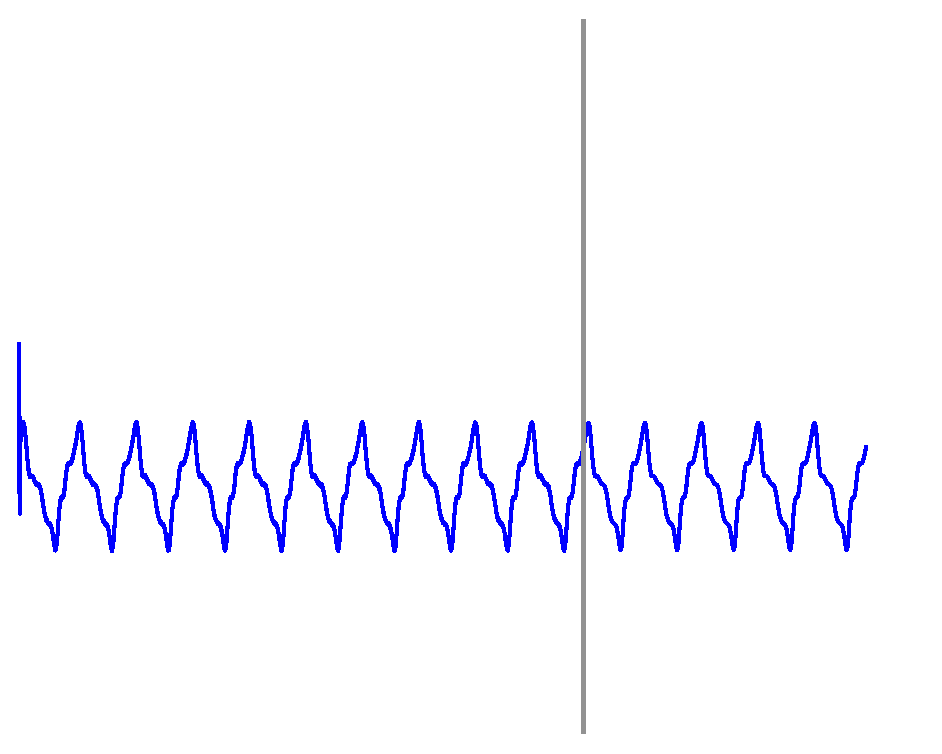
\includegraphics[height=0.1\linewidth,width=.45\linewidth]{Figures/Fig_T3/MATLAB/ST_T2_Seg2_Theta0.eps}
        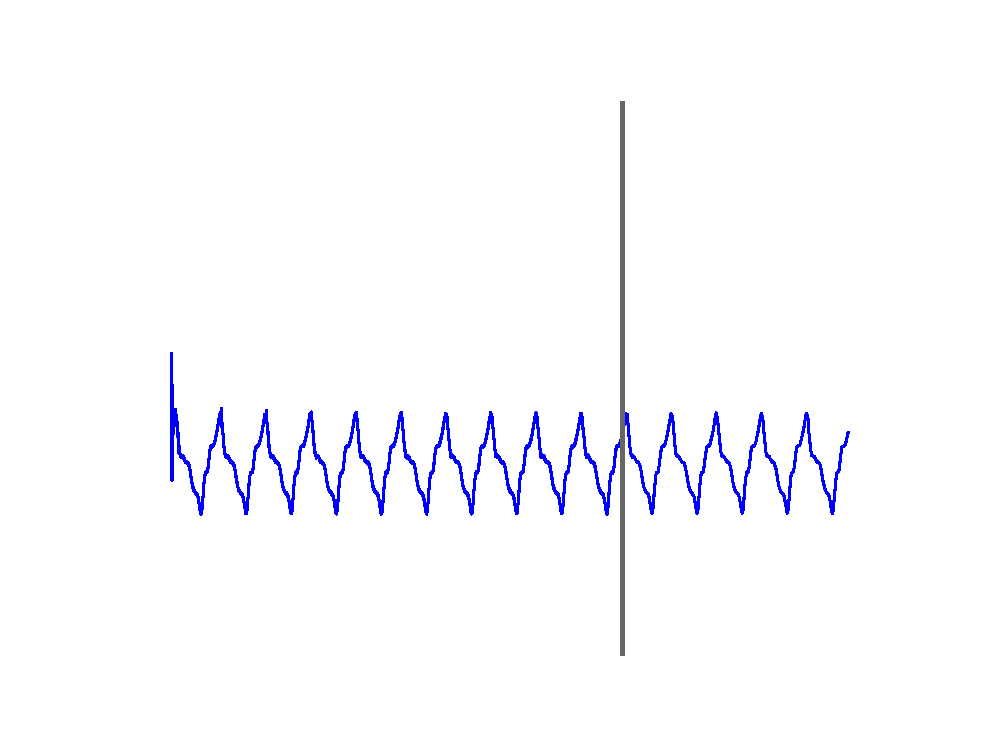
\includegraphics[trim=2cm 1cm 2cm 1cm, clip=true,height=0.1\linewidth,width=.45\linewidth]{Figures/Fig_T3/Python/ST_T2_Seg2_Theta0.eps}
        
        \end{subfigure}
        
        
        \textbf{\rotatebox[origin=c]{90}{$\theta_2$}}\begin{subfigure}{\textwidth}
        \centering
        
        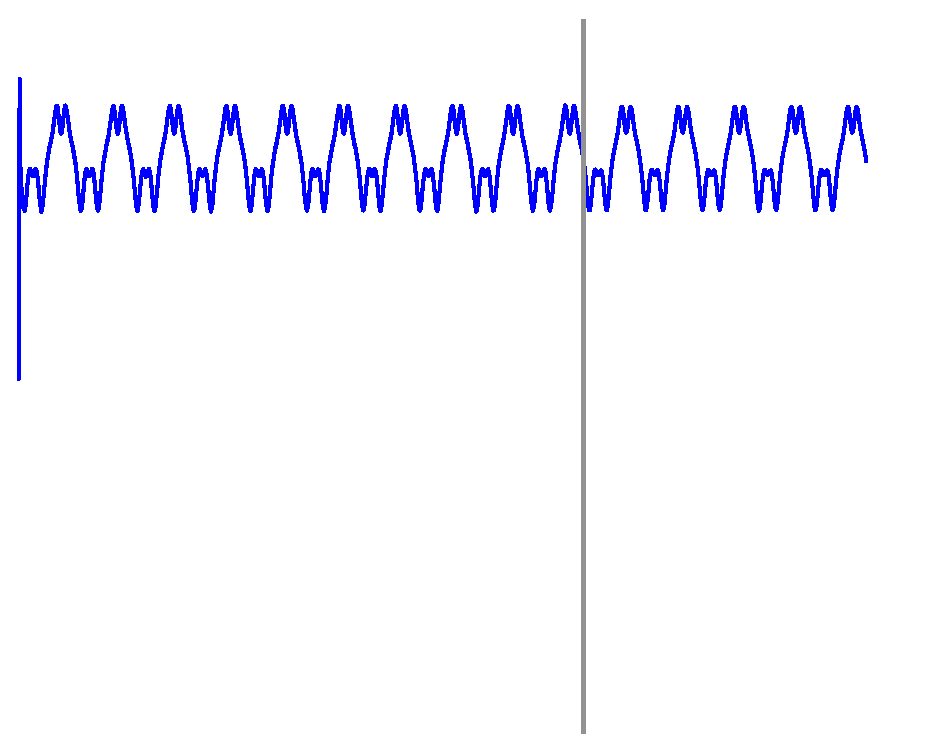
\includegraphics[height=0.1\linewidth,width=.45\linewidth]{Figures/Fig_T3/MATLAB/ST_T2_Seg2_Theta1.eps}
        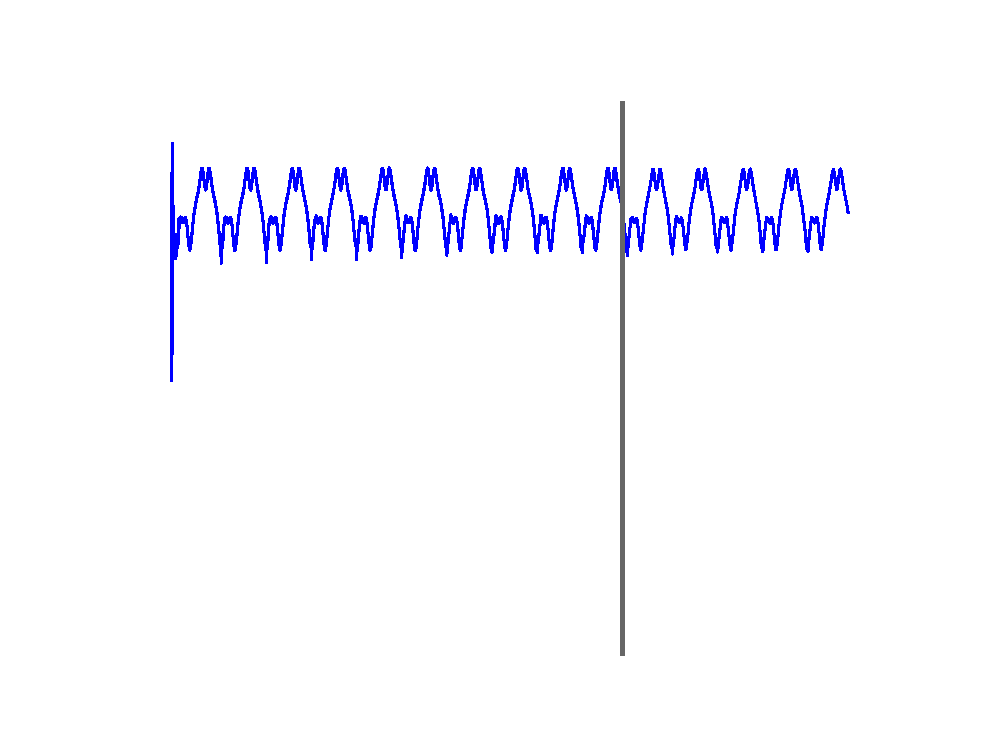
\includegraphics[trim=2cm 1cm 2cm 1cm, clip=true,height=0.1\linewidth,width=.45\linewidth]{Figures/Fig_T3/Python/ST_T2_Seg2_Theta1.eps}
        
        \end{subfigure}
         
        
        \textbf{\rotatebox[origin=c]{90}{MSE}}\begin{subfigure}{\textwidth}
        \centering
        
        \hspace{-2em}
        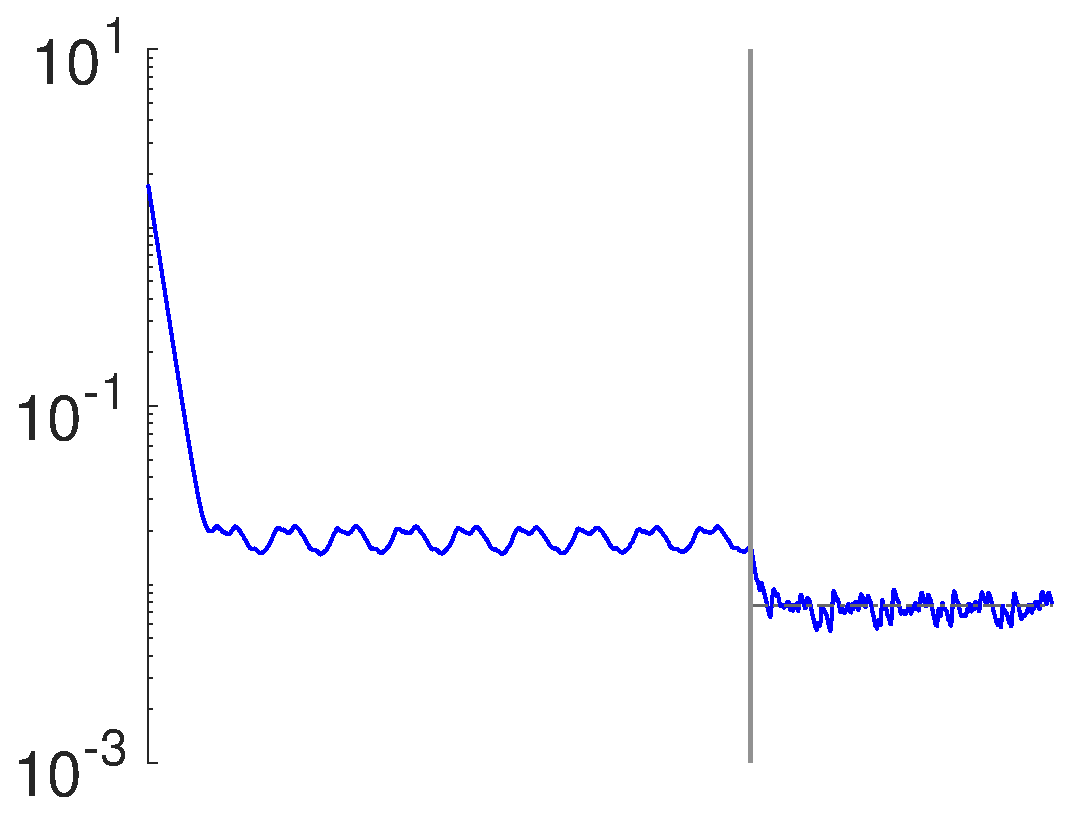
\includegraphics[height=0.15\linewidth,width=.45\linewidth]{Figures/Fig_T3/MATLAB/ST_T2_Seg2_MSE.eps}
        \hspace{.5em}
        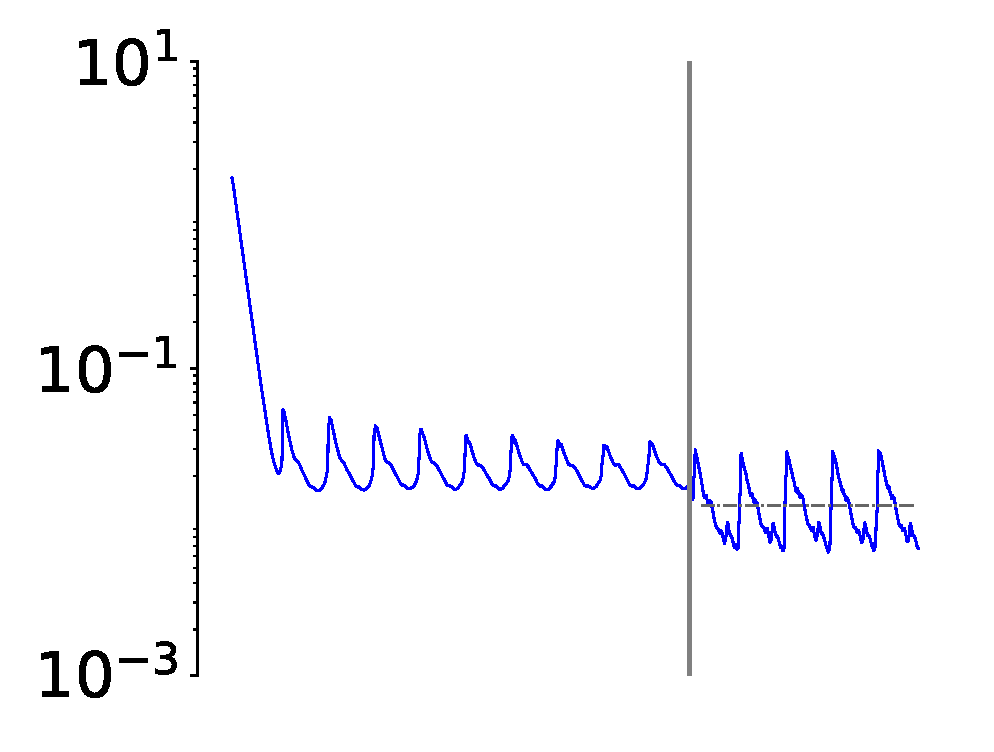
\includegraphics[height=0.15\linewidth,width=.45\linewidth]{Figures/Fig_T3/Python/ST_T2_Seg2_MSE.eps}
        
        \end{subfigure}
        

        
        
        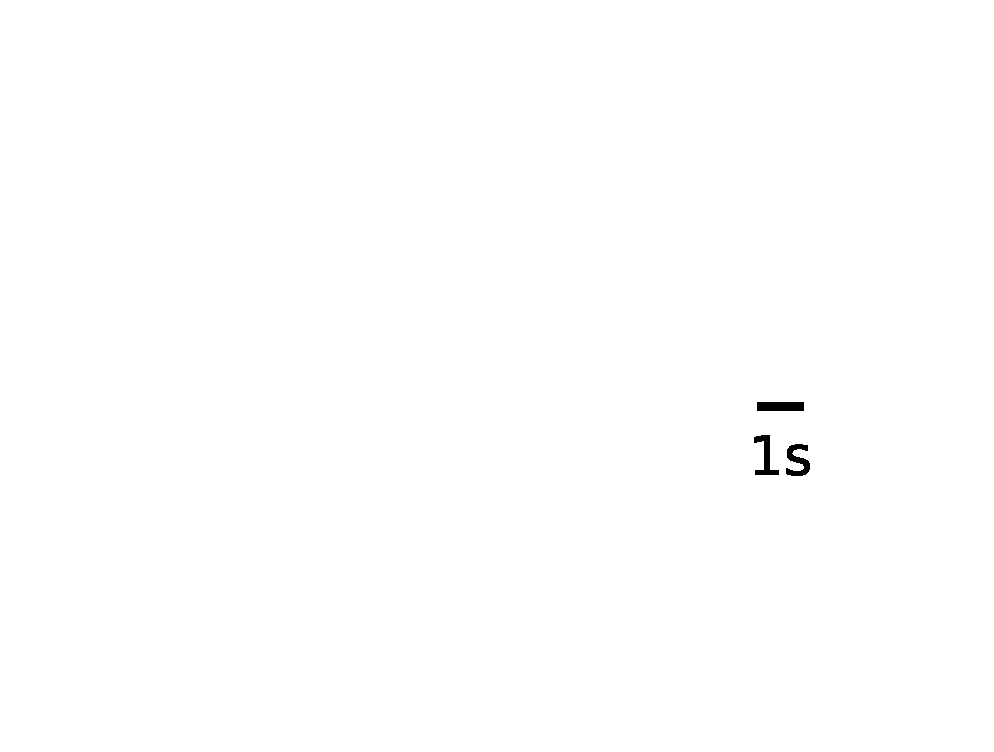
\includegraphics[trim=2cm 6cm 2cm 6cm, clip=true,height=0.05\linewidth,width=.4\linewidth]{Figures/Fig_T1/Python/ST_T1_Scale.eps}
        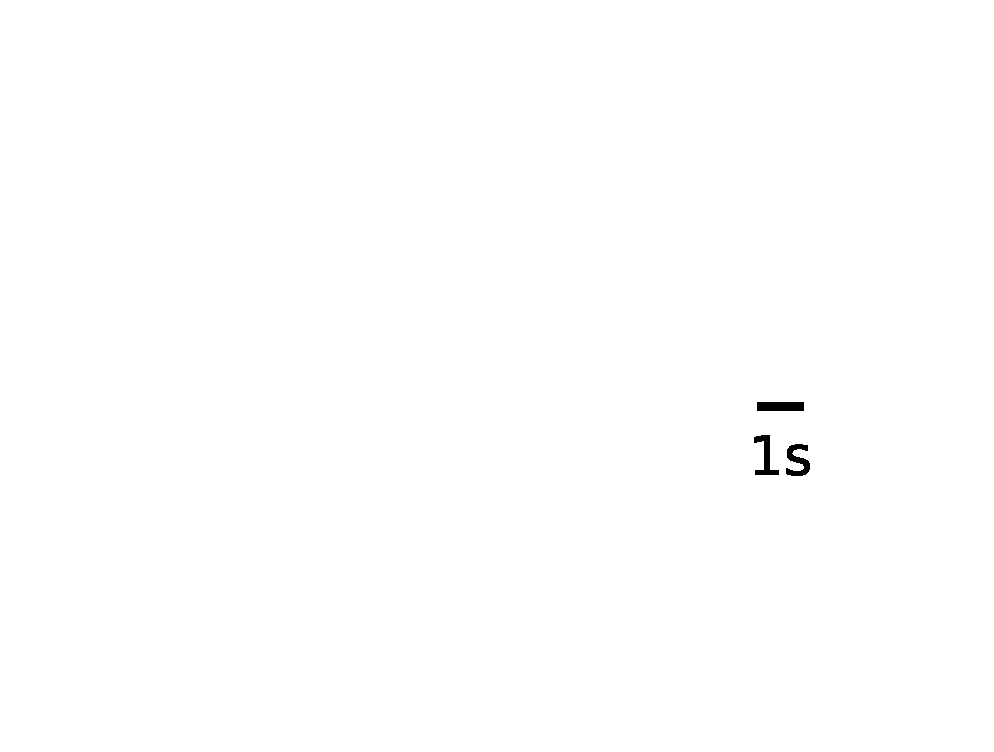
\includegraphics[trim=2cm 4cm 2cm 6cm, clip=true,height=0.05\linewidth,width=.45\linewidth]{Figures/Fig_T1/Python/ST_T1_Scale.eps}
        
        
    \caption{Results for Task 2 with the SUPERTREX algorithm. The target time‐series is learned accurately during the training phase, and is also maintained in a stable manner, during the testing phase, in both implementations, as presented in \cite{pyle2019}.}
    \label{Fig:compTask2ST}
    
    \end{subfigure}


\caption{Comparison of the performances of original scripts (left column) and Python adaptation (right column) with the results presented in the original article (center column), for the RMHL and SUPERTREX, on Task 2 \cite{pyle2019}. All simulations shown here use the MATLAB default (5489) as the seed for the random number generator. In each subfigure, the top row shows the target trajectory (red) with the trajectory generated by the algorithm (blue) throughout the test phase. The second row shows the time-series (blue) generated by the model (joint angles ($\theta_i$), in this case). The bottom row shows the distance from target metric (blue) over the simulation (x and y coordinates, in this case), using the log scale for the y axis. The horizontal grey line, in the test phase, indicates the deviation metric. The grey vertical line marks the separation of the training and testing phase.}
\label{Fig:Comparison_Task2}

\end{figure}